\pdfminorversion=4
\documentclass{beamer}
\usepackage{amssymb}
\usepackage{mathpazo}
\usepackage{multimedia}
\usepackage{amsfonts}
\usepackage{amsmath}
\usepackage{hyperref}
\usepackage{graphicx}
\usepackage{listings}

\setcounter{MaxMatrixCols}{10}

\hypersetup{
colorlinks = true,
allcolors = blue,
}
\definecolor{mygreen}{rgb}{0,0.6,0}
\newtheorem{prop}{Proposition}
\newcommand{\E}{\mathbb{E}}
\newcommand{\eps}{\varepsilon}
\setbeamertemplate{footline}[frame number]
\setbeamertemplate{navigation symbols}{}
\setbeamertemplate{mini frames}{}
\setbeamertemplate{itemize item}[ball]
\setbeamertemplate{itemize subitem}[ball]
\setbeamercovered{invisible}
\newcommand{\beginbackup}{
   \newcounter{framenumbervorappendix}
   \setcounter{framenumbervorappendix}{\value{framenumber}}
}
\newcommand{\backupend}{
   \addtocounter{framenumbervorappendix}{-\value{framenumber}}
   \addtocounter{framenumber}{\value{framenumbervorappendix}}
}
\renewcommand{\baselinestretch}{1.2}
\small\normalsize
\institute[University of Birmingham]{University of Birmingham}

\begin{document}

\title{Advanced Numerical Methods}
\subtitle{Solving DSGE Models with Dynare, Part 1}
\author{Alessandro~Di Nola}
\date{}

\begin{frame}
\titlepage
\end{frame}
%%%%%%%%%%%%%%%%%%%%%%%%%%%%%%%%%%%%%%%%%%%%%%%%%%%%%%%%

\begin{frame}
\frametitle{Outline}

\begin{itemize}
\item The stochastic growth model: quick review
\item Equilibrium conditions and deterministic steady state
\item Approximation with first-order perturbation
\item Solution by undetermined coefficients
\item Simulation and impulse responses
\item MATLAB implementation
\end{itemize}

\end{frame}
%%%%%%%%%%%%%%%%%%%%%%%%%%%%%%%%%%%%%%%%%%%%%%%%%%%%%%%%

\begin{frame}
\frametitle{The Stochastic Growth Model}

\begin{itemize}
\item We solve the stochastic neoclassical growth model using the first-order perturbation method.
\item The workflow is:
\begin{enumerate}
\item Write down the equilibrium conditions.
\item Compute the deterministic steady state.
\item Take a linear or log-linear approximation around the deterministic steady state.
\item Solve the linear rational expectations system with the method of undetermined coefficients (main reference: \hyperlink{ref:uhlig}{Uhlig, 1999})
\item Simulate the model and compute impulse responses.
\end{enumerate}
\item We will see later how to \textcolor{red}{automate} these steps with \textcolor{red}{Dynare}.
\end{itemize}

\end{frame}
%%%%%%%%%%%%%%%%%%%%%%%%%%%%%%%%%%%%%%%%%%%%%%%%%%%%%%%%

\begin{frame}
\frametitle{Step 1 - The Planner's Problem}

\begin{itemize}	
\item The planner chooses the sequence $\{c_t,k_{t+1}\}_{t=0}^{\infty}$ to solve
\begin{equation*}
\max_{\{c_t,k_{t+1}\}_{t=0}^{\infty}}
\;
E_0\left\{\sum_{t=0}^{\infty}\beta^t \frac{c_t^{1-\sigma}}{1-\sigma}\right\}
\end{equation*}
subject to
\begin{equation*}
c_t + k_{t+1} \le z_t k_t^\alpha + (1-\delta)k_t,
\qquad t=0,1,2,\dots
\end{equation*}
\item $c_t$ is consumption, $k_t$ is beginning-of-period capital, and $z_t$ is productivity.
\item Parameters: $\beta \in (0,1)$, $\sigma > 0$, $\alpha \in (0,1)$, $\delta \in (0,1]$.
\pause 
\item \textcolor{red}{Q}: Why do we consider the planner's problem if we are ultimately interested in a competitive equilibrium?
\end{itemize}

\end{frame}
%%%%%%%%%%%%%%%%%%%%%%%%%%%%%%%%%%%%%%%%%%%%%%%%%%%%%%%%

\begin{frame}
\hypertarget{euler-main}{}
\frametitle{Step 1 - Technology and First-Order Conditions}

\begin{itemize}
\item Productivity follows
\begin{equation*}
\log z_{t+1} = \rho \log z_t + \varepsilon_{t+1},
\qquad
\varepsilon_{t+1} \sim \text{i.i.d. } N(0,\sigma_\varepsilon^2)
\end{equation*}
with $\rho \in (0,1)$.
\item The first-order conditions w.r.t. $c_t$ and $k_{t+1}$ are
\begin{equation*}
c_t^{-\sigma} = \lambda_t
\end{equation*}
\begin{equation*}
\lambda_t = \beta E_t\left[
\lambda_{t+1}\left(\alpha z_{t+1}k_{t+1}^{\alpha-1} + 1-\delta\right)
\right]
\end{equation*}
where $\lambda_t$ is the Lagrange multiplier on the resource constraint.
\hyperlink{euler-derivation}{\beamerbutton{Derivation}}
\item These conditions hold together with the resource constraint.
\end{itemize}

\end{frame}
%%%%%%%%%%%%%%%%%%%%%%%%%%%%%%%%%%%%%%%%%%%%%%%%%%%%%%%%

\begin{frame}
\frametitle{Step 1 - Equilibrium Conditions}

\begin{itemize}
\item There are \textcolor{blue}{three endogenous variables}:
\[
c_t,\qquad k_t,\qquad z_t.
\]
\item Therefore we must have \textcolor{blue}{three equilibrium equations}.
\item Among the endogenous variables, $k_t$ and $z_t$ are state variables, while $c_t$ is the control variable.
\item $\varepsilon_t$ is an \textcolor{red}{exogenous shock}.
\item The equilibrium system is
\begin{equation}\tag{EE}\label{eq:euler}
	c_t^{-\sigma} = \beta E_t\left[
	c_{t+1}^{-\sigma}\left(\alpha z_{t+1}k_{t+1}^{\alpha-1}+1-\delta\right)
	\right]
\end{equation}
\begin{equation}\tag{RC}\label{eq:rc}
c_t + k_{t+1} = z_t k_t^\alpha + (1-\delta)k_t
\end{equation}
\begin{equation}\tag{Shock}\label{eq:shock}
\log z_t = \rho \log z_{t-1} + \varepsilon_t,
\qquad
\varepsilon_t \sim \text{i.i.d. } N(0,\sigma_\varepsilon^2)
\end{equation}
\end{itemize}

\end{frame}
%%%%%%%%%%%%%%%%%%%%%%%%%%%%%%%%%%%%%%%%%%%%%%%%%%%%%%%%

\begin{frame}
\frametitle{Step 2 - Deterministic Steady State}

\begin{itemize}
\item In the deterministic steady state, $\varepsilon_t=0$ and 
\[
c_t=\bar c,\qquad k_t=\bar k,\qquad z_t=\bar z
\]
for all $t$.
\item The steady-state system is
\begin{equation}\tag{EE-SS}\label{eq:euler_ss}
1 = \beta\left(\alpha \bar z \bar k^{\alpha-1} + 1-\delta\right) 
\end{equation}
\begin{equation}\tag{RC-SS}\label{eq:rc_ss}
\bar c + \bar k = \bar z \bar k^\alpha + (1-\delta)\bar k
\end{equation}
\begin{equation}\tag{Shock-SS}\label{eq:shock_ss}
\log \bar z = \rho \log \bar z
\end{equation}
\item Since $\rho \in (0,1)$, we have $\bar z = 1$.
\end{itemize}

\end{frame}
%%%%%%%%%%%%%%%%%%%%%%%%%%%%%%%%%%%%%%%%%%%%%%%%%%%%%%%%

\begin{frame}
\frametitle{Step 3 - Steady-State Capital and Consumption}

\begin{itemize}
\item Solving (\ref{eq:euler_ss}) for steady-state capital,
\begin{equation}
\bar k =
\left(
\frac{\alpha \bar z}{\frac{1}{\beta}-1+\delta}
\right)^{\frac{1}{1-\alpha}}
\label{eq:ss_k_slide}
\end{equation}
\item Steady-state consumption follows from (\ref{eq:rc_ss})
\begin{equation}
\bar c = \bar z \bar k^\alpha - \delta \bar k
\label{eq:ss_c_slide}
\end{equation}
\item Steady-state output is
\begin{equation}
\bar y = \bar z \bar k^\alpha
\label{eq:ss_y_slide}
\end{equation}
\end{itemize}

\end{frame}
%%%%%%%%%%%%%%%%%%%%%%%%%%%%%%%%%%%%%%%%%%%%%%%%%%%%%%%%

\begin{frame}
\frametitle{Step 3 - First-Order Approximation}

\begin{itemize}
\item If $f(x_t,y_t)=0$, a first-order Taylor approximation around $(\bar x,\bar y)$ is
\begin{equation*}
f(x_t,y_t)
\approx
f(\bar x,\bar y)
+ f_x(\bar x,\bar y)(x_t-\bar x)
+ f_y(\bar x,\bar y)(y_t-\bar y)
\end{equation*}
\item Define log deviations as
\begin{equation*}
\hat x_t \equiv \log\left(\frac{x_t}{\bar x}\right)
\approx \frac{x_t-\bar x}{\bar x}
\end{equation*}
\item A useful rule is
\begin{equation*}
x_t = \bar x e^{\hat x_t} \approx \bar x(1+\hat x_t)
\end{equation*}
\end{itemize}

\end{frame}
%%%%%%%%%%%%%%%%%%%%%%%%%%%%%%%%%%%%%%%%%%%%%%%%%%%%%%%%

\begin{frame}
\frametitle{Step 3 - Linearized Resource Constraint}

\begin{itemize}
\item Define
\begin{equation*}
\hat c_t = \log\left(\frac{c_t}{\bar c}\right),
\qquad
\hat k_t = \log\left(\frac{k_t}{\bar k}\right),
\qquad
\hat z_t = \log\left(\frac{z_t}{\bar z}\right)
\end{equation*}
\item The log-linearized resource constraint is
\begin{equation}\tag{RC-LIN}\label{eq:rc_lin}
\frac{\bar c}{\bar k}\hat c_t + \hat k_{t+1}
- \frac{1}{\beta}\hat k_t
- \frac{1}{\alpha}\left(\frac{1}{\beta}-1+\delta\right)\hat z_t
= 0
\end{equation}
\item Here
\begin{equation*}
\frac{\bar y}{\bar k} = \bar z \bar k^{\alpha-1}
= \frac{1}{\alpha}\left(\frac{1}{\beta}-1+\delta\right)
\end{equation*}
\end{itemize}

\end{frame}
%%%%%%%%%%%%%%%%%%%%%%%%%%%%%%%%%%%%%%%%%%%%%%%%%%%%%%%%

\begin{frame}
\frametitle{Step 3 - Linearized Euler Equation}
\begin{itemize}
\item Define the gross return on capital and its log deviation:
\begin{equation*}
\begin{aligned}
R_{t+1} \equiv \alpha z_{t+1}k_{t+1}^{\alpha-1}+1-\delta
\qquad
\hat R_{t+1} \equiv \frac{R_{t+1}-\bar R}{\bar R}
\end{aligned}
\end{equation*}
\item Since $\bar R = 1/\beta$, a first-order approximation of the Euler equation implies
\begin{equation}
\hat c_t = E_t \hat c_{t+1} - \frac{1}{\sigma} E_t \hat R_{t+1}
\end{equation}
\item Also,
\begin{equation}
\hat R_{t+1}
=
\left[1-\beta(1-\delta)\right]
\left(\hat z_{t+1}-(1-\alpha)\hat k_{t+1}\right)
\end{equation}
\item Using $E_t \hat z_{t+1}=\rho \hat z_t$, the linearized Euler equation becomes
\small
\begin{equation}\tag{EE-LIN}\label{eq:ee_lin}
\hat c_t = E_t\hat c_{t+1} - \frac{1}{\sigma}\left[1-\beta(1-\delta)\right]\rho \hat z_t + \frac{1}{\sigma}(1-\alpha)\left[1-\beta(1-\delta)\right]\hat k_{t+1}
\end{equation}
\normalsize
\end{itemize}

\end{frame}
%%%%%%%%%%%%%%%%%%%%%%%%%%%%%%%%%%%%%%%%%%%%%%%%%%%%%%%%

\begin{frame}
\frametitle{Step 3 - The Linear System}

\begin{itemize}
\item The linearized model is given by (\ref{eq:rc_lin})-(\ref{eq:ee_lin}): 
\begin{equation*}
\alpha_1 \hat c_t + \alpha_2 \hat k_{t+1} + \alpha_3 \hat k_t + \alpha_4 \hat z_t = 0
\end{equation*}
\begin{equation*}
\beta_1 \hat c_t + \beta_2 E_t\hat c_{t+1} + \beta_3 \hat z_t + \beta_4 \hat k_{t+1} = 0
\end{equation*}
\item where
\begin{equation*}
\begin{aligned}
\alpha_1 &= \frac{\bar c}{\bar k},\quad
\alpha_2 = 1,\\
\alpha_3 &= -\frac{1}{\beta},\quad
\alpha_4 = -\frac{1}{\alpha}\left(\frac{1}{\beta}-1+\delta\right)
\end{aligned}
\end{equation*}
\begin{equation*}
\begin{aligned}
\beta_1 &= 1,\quad
\beta_2 = -1,\\
\beta_3 &= \frac{1}{\sigma}\left[1-\beta(1-\delta)\right]\rho,\quad
\beta_4 = -\frac{1}{\sigma}(1-\alpha)\left[1-\beta(1-\delta)\right]
\end{aligned}
\end{equation*}
\end{itemize}

\end{frame}
%%%%%%%%%%%%%%%%%%%%%%%%%%%%%%%%%%%%%%%%%%%%%%%%%%%%%%%%

\begin{frame}
\frametitle{Step 4 - Policy Functions}

\begin{itemize}
\item Guess \textcolor{red}{linear} decision (policy) rules:
\begin{equation}\tag{POL-C}\label{eq:pol_c}
\hat c_t = \eta_{ck}\hat k_t + \eta_{cz}\hat z_t
\end{equation}
\begin{equation}\tag{POL-K}\label{eq:pol_k}
\hat k_{t+1} = \eta_{kk}\hat k_t + \eta_{kz}\hat z_t
\end{equation}
\item Taking expectations,
\begin{equation*}
E_t \hat c_{t+1}
= \eta_{ck}\eta_{kk}\hat k_t
+ \left(\eta_{ck}\eta_{kz}+\eta_{cz}\rho\right)\hat z_t
\end{equation*}
\end{itemize}
\textbf{Procedure}:
\begin{itemize}
\item Substitute (\ref{eq:pol_c})-(\ref{eq:pol_k}) into the two linearized equilibrium equations.
\item Resulting expressions must hold for every possible value of the state variables $\hat k_t$ and $\hat z_t$.
\item Therefore, in each equation, the coefficient on $\hat k_t$ must be zero and the coefficient on $\hat z_t$ must also be zero.
\item This gives four equations for the four unknown coefficients
\[
\eta_{ck},\quad \eta_{cz},\quad \eta_{kk},\quad \eta_{kz}.
\]
\end{itemize}

\end{frame}
%%%%%%%%%%%%%%%%%%%%%%%%%%%%%%%%%%%%%%%%%%%%%%%%%%%%%%%%

\begin{frame}
\frametitle{Step 4 - Undetermined Coefficients}
\small
\begin{equation}
\alpha_1\eta_{ck}+\alpha_2\eta_{kk}+\alpha_3=0
\tag{UC-1} \label{eq:und_slide_1}
\end{equation}
\begin{equation}
\alpha_1\eta_{cz}+\alpha_2\eta_{kz}+\alpha_4=0
\tag{UC-2} \label{eq:und_slide_2}
\end{equation}
\begin{equation}
\beta_1\eta_{ck}+\beta_2\eta_{ck}\eta_{kk}+\beta_4\eta_{kk}=0
\tag{UC-3} \label{eq:und_slide_3}
\end{equation}
\begin{equation}
\beta_1\eta_{cz}
+ \beta_2\left(\eta_{ck}\eta_{kz}+\eta_{cz}\rho\right)
+ \beta_3
+ \beta_4\eta_{kz}=0
\tag{UC-4} \label{eq:und_slide_4}
\end{equation}

\begin{itemize}
\item From equation \eqref{eq:und_slide_1} we have
\end{itemize}
\begin{equation}
\eta_{ck} = -\frac{\alpha_2\eta_{kk}+\alpha_3}{\alpha_1}
\tag{eta-ck} \label{eq:eta_ck_slide}
\end{equation}

\begin{itemize}
\item Substituting \eqref{eq:eta_ck_slide} into equation \eqref{eq:und_slide_3}, we obtain the \textcolor{red}{quadratic equation} for $\eta_{kk}$:
\end{itemize}
\begin{equation*}
\beta_2\alpha_2\eta_{kk}^2
+ \left(\beta_1\alpha_2+\beta_2\alpha_3-\beta_4\alpha_1\right)\eta_{kk}
+ \beta_1\alpha_3
= 0
\end{equation*}

\end{frame}
%%%%%%%%%%%%%%%%%%%%%%%%%%%%%%%%%%%%%%%%%%%%%%%%%%%%%%%%

\begin{frame}
	\frametitle{Step 4 - Stable and Unstable Root}
	
\begin{itemize}
	\item Quadratic equation for $\eta_{kk}$:
	\begin{equation*}
		P(\eta_{kk})\equiv \beta_2\alpha_2\eta_{kk}^2
		+ \left(\beta_1\alpha_2+\beta_2\alpha_3-\beta_4\alpha_1\right)\eta_{kk}
		+ \beta_1\alpha_3
		= 0
	\end{equation*}
	\item It can be shown that this equation has two roots: one root with modulus less than 1 (\textcolor{blue}{stable}) and the other with modulus greater than 1 (\textcolor{red}{unstable}).
\end{itemize}

\begin{center}
	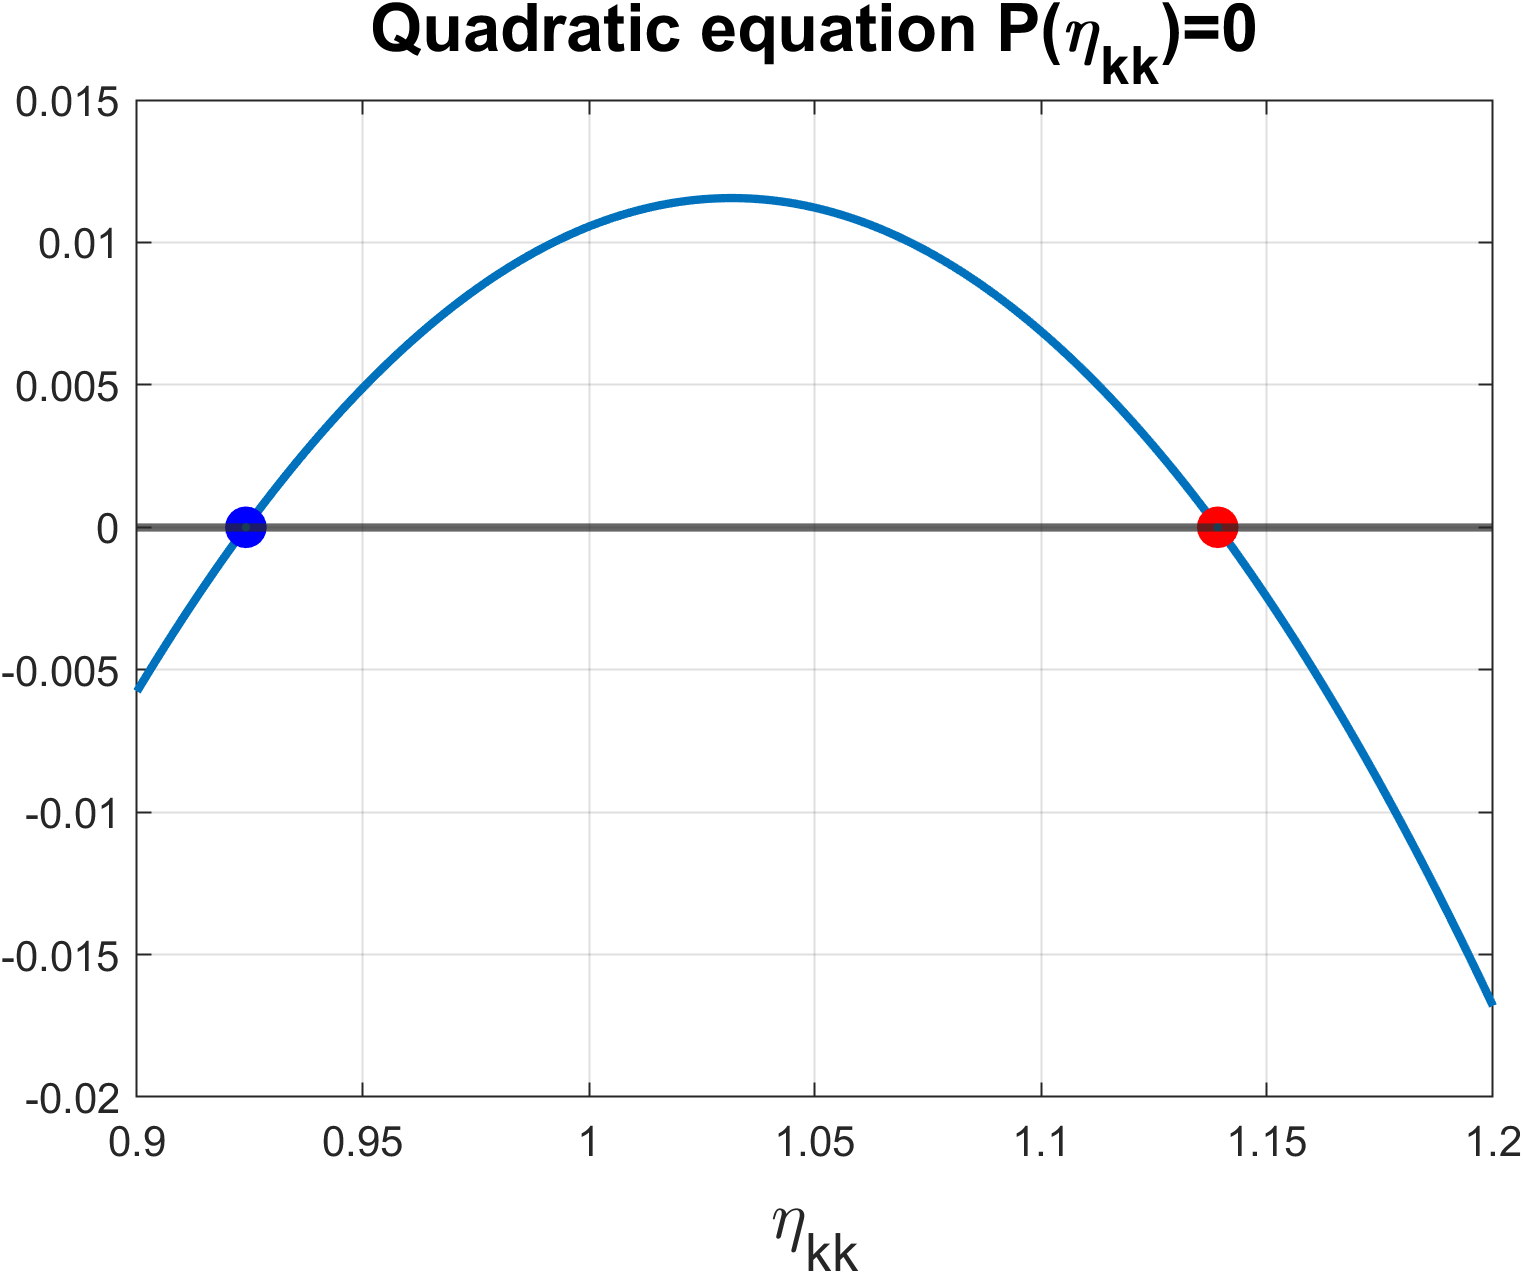
\includegraphics[width=0.5\textwidth]{../figs/quadratic.png}
\end{center}
	
\end{frame}
%%%%%%%%%%%%%%%%%%%%%%%%%%%%%%%%%%%%%%%%%%%%%%%%%%%%%%%%

\begin{frame}
\frametitle{Step 4 - Closed-Form Coefficients}
\small
\begin{itemize}
\item Select the stable root of the quadratic, the one satisfying $|\eta_{kk}|<1$.
\item Then recover the remaining coefficients:
\begin{equation*}
\eta_{cz} = -\frac{\alpha_2\eta_{kz}+\alpha_4}{\alpha_1}
\end{equation*}
\begin{equation*}
\eta_{kz}
=
\frac{\left(\beta_1+\rho\beta_2\right)\alpha_4-\alpha_1\beta_3}
{\alpha_1\beta_4-\beta_1\alpha_2+\beta_2\left(\alpha_1\eta_{ck}-\alpha_2\rho\right)}
\end{equation*}
\item Once we have the four coefficients, we can simulate the model and compute impulse responses.
\end{itemize}

\end{frame}
%%%%%%%%%%%%%%%%%%%%%%%%%%%%%%%%%%%%%%%%%%%%%%%%%%%%%%%%

\begin{frame}
\frametitle{Step 5 - Simulation and Impulse Responses}

\begin{itemize}
\item Start from $\hat z_0=0$ and $\hat k_0=0$.
\item For simulations, generate shocks $\{\varepsilon_t\}_{t=1}^T$ from $N(0,\sigma_\varepsilon^2)$ and use
\begin{equation*}
\hat z_t = \rho \hat z_{t-1} + \varepsilon_t
\end{equation*}
\item Iterate on the policy rules:
\begin{equation*}
\hat c_t = \eta_{ck}\hat k_t + \eta_{cz}\hat z_t,
\qquad
\hat k_{t+1} = \eta_{kk}\hat k_t + \eta_{kz}\hat z_t
\end{equation*}
\item Recover output from
\begin{equation*}
\hat y_t = \hat z_t + \alpha \hat k_t
\end{equation*}
\end{itemize}

\end{frame}
%%%%%%%%%%%%%%%%%%%%%%%%%%%%%%%%%%%%%%%%%%%%%%%%%%%%%%%%

\begin{frame}
\frametitle{Impulse Response from MATLAB}
\begin{center}
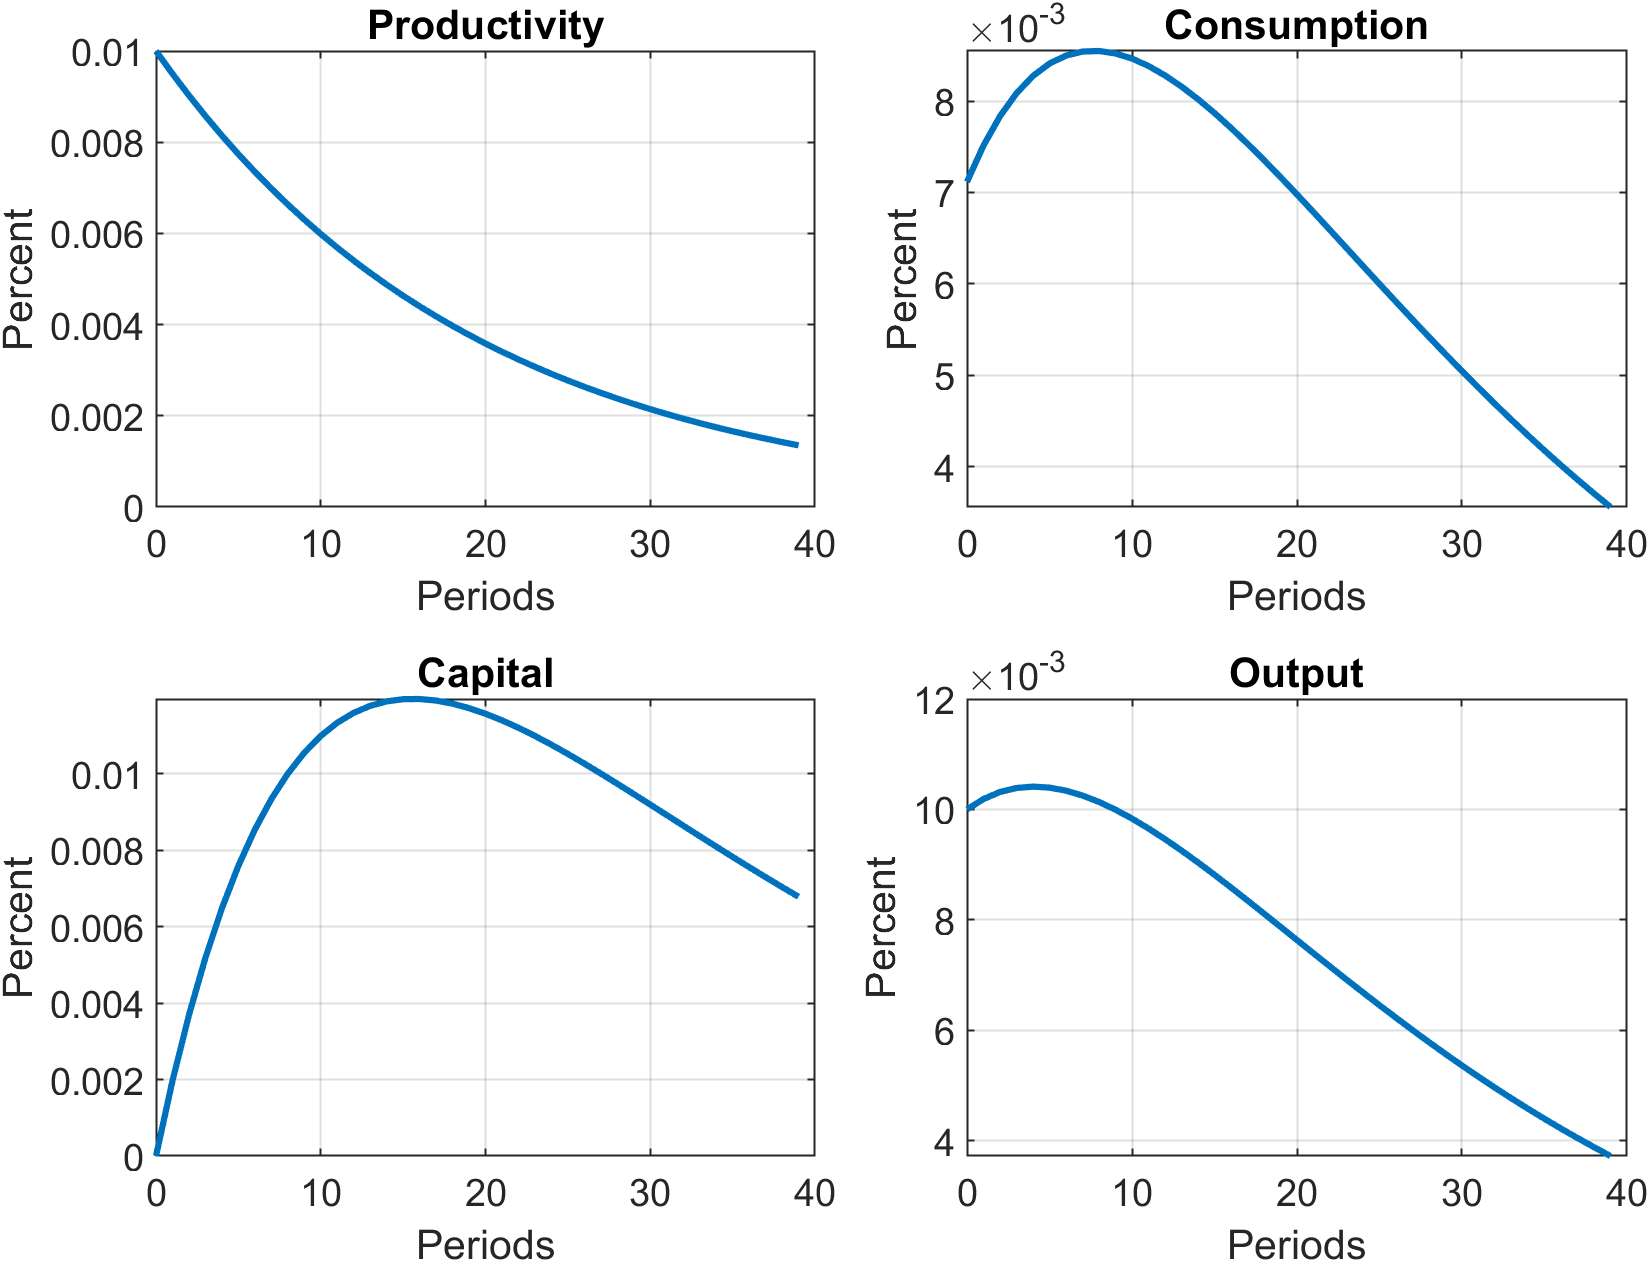
\includegraphics[width=0.92\textwidth]{../figs/undet_coeffs_irf.png}
\end{center}
\end{frame}
%%%%%%%%%%%%%%%%%%%%%%%%%%%%%%%%%%%%%%%%%%%%%%%%%%%%%%%%

\begin{frame}
\frametitle{Stochastic Simulation from MATLAB}
\begin{center}
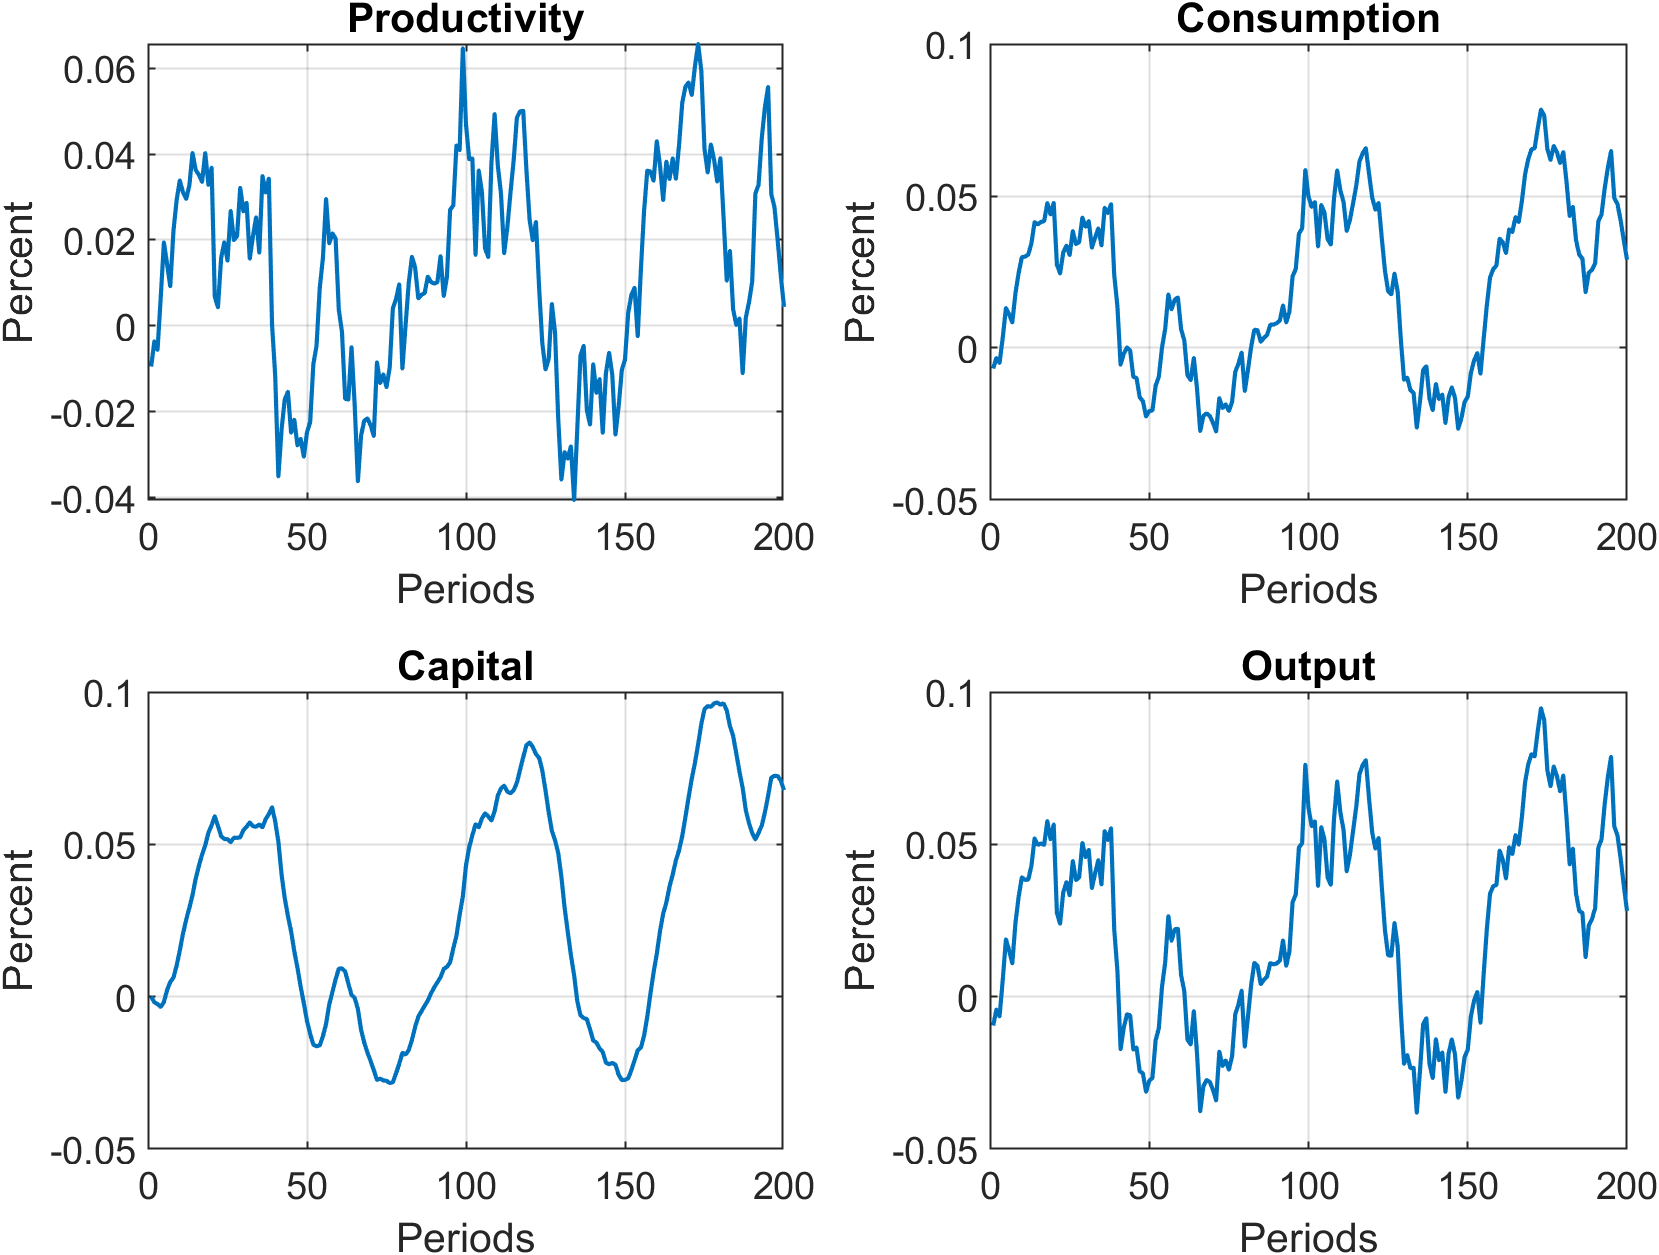
\includegraphics[width=0.92\textwidth]{../figs/undet_coeffs_simulation.png}
\end{center}
\end{frame}
%%%%%%%%%%%%%%%%%%%%%%%%%%%%%%%%%%%%%%%%%%%%%%%%%%%%%%%%

\begin{frame}[fragile]
\frametitle{MATLAB Implementation}
\small
\begin{itemize}
\item The teaching script is \texttt{codes/main\_undet\_coeffs.m}.
\item It follows exactly the structure of the notes:
\begin{enumerate}
\item set parameters,
\item compute the steady state,
\item build the linear coefficients,
\item solve for $\eta_{ck},\eta_{cz},\eta_{kk},\eta_{kz}$,
\item produce an IRF and a stochastic simulation.
\end{enumerate}
\item The auxiliary function \texttt{codes/fun\_ss.m} computes
\[
\bar k,\quad \bar c,\quad \bar z,\quad \bar y.
\]
\end{itemize}

\end{frame}
%%%%%%%%%%%%%%%%%%%%%%%%%%%%%%%%%%%%%%%%%%%%%%%%%%%%%%%%

\beginbackup

\begin{frame}
\hypertarget{euler-derivation}{}
\frametitle{Appendix: Euler Equation Derivation}

\begin{itemize}
	\item Consider the planner's problem:
	\begin{equation*}
	\max_{\{c_{t},k_{t+1}\}} \mathbb{E}_{0}\sum_{t=0}^{\infty }\beta ^{t}\frac{c_{t}^{1-\sigma }}{1-\sigma }
	\end{equation*}
	subject to
	\begin{equation*}
	c_{t}+k_{t+1}=z_{t}k_{t}^{\alpha }+(1-\delta )k_{t}.
	\end{equation*}

	\item Attach multiplier $\lambda_t$ to the resource constraint. The intertemporal Lagrangian is
	\begin{equation*}
	\mathcal{L}=\mathbb{E}_{0}\sum_{t=0}^{\infty }\beta ^{t}\left[
	\frac{c_{t}^{1-\sigma }}{1-\sigma }+\lambda _{t}\left( z_{t}k_{t}^{\alpha }+(1-\delta )k_{t}-c_{t}-k_{t+1}\right) \right] .
	\end{equation*}
\end{itemize}
\end{frame}

\begin{frame}
\frametitle{Appendix: Euler Equation Derivation}

\begin{itemize}
	\item FOC with respect to $c_t$:
	\begin{equation*}
	\frac{\partial \mathcal{L}}{\partial c_{t}}:\quad c_{t}^{-\sigma }-\lambda _{t}=0
	\quad \Rightarrow \quad \lambda _{t}=c_{t}^{-\sigma }.
	\end{equation*}

	\item FOC with respect to $k_{t+1}$:
	\begin{equation*}
	\frac{\partial \mathcal{L}}{\partial k_{t+1}}:\quad -\lambda _{t}+\beta E_t\left[ \lambda _{t+1}\left( \alpha z_{t+1}k_{t+1}^{\alpha -1}+1-\delta \right) \right] =0.
	\end{equation*}

	\item Substitute out the multiplier using $\lambda _{t}=c_{t}^{-\sigma }$ and $\lambda _{t+1}=c_{t+1}^{-\sigma }$:
	\begin{equation*}
	c_{t}^{-\sigma }=\beta E_t\left[ c_{t+1}^{-\sigma }\left(
	\alpha z_{t+1}k_{t+1}^{\alpha -1}+1-\delta \right) \right] .
	\end{equation*}

	\item This is the Euler equation in the main text.
	\hyperlink{euler-main}{\beamerbutton{back}}
\end{itemize}
\end{frame}

\backupend

%%%%%%%%%%%%%%%%%%%%%%%%%%%%%%%%%%%%%%%%%%%%%%%%%%%%%%%%

\begin{frame}
\frametitle{References}

\small

\begin{itemize}
	\item \hypertarget{ref:uhlig}{Uhlig, H. (1999). ``A Toolkit for Analyzing Nonlinear Dynamic Stochastic Models Easily.''} In R. Marimon and A. Scott (eds.), \textit{Computational Methods for the Study of Dynamic Economies}, Oxford University Press, 30--61.
	
	\item Miao, J. (2020). \textit{Economic Dynamics in Discrete Time}, 2nd ed. Cambridge, MA: The MIT Press.
\end{itemize}


\end{frame}
%%%%%%%%%%%%%%%%%%%%%%%%%%%%%%%%%%%%%%%%%%%%%%%%%%%%%%%%

\end{document}
